\documentclass[a4paper,12pt]{article}
\usepackage{graphicx}
\usepackage{amsmath}
\usepackage{amssymb}
\usepackage{listings}
\usepackage{xcolor}
\usepackage{caption}
\usepackage{subcaption}
\usepackage{float}
\usepackage{geometry}
\geometry{margin=1in}
\usepackage{hyperref}
\usepackage{url} % Improved URL formatting

\title{\centering \textbf{ENPM 701 - Homework 1}}
\author{Neeraj Laul\\UID 120518973}
\date{\today}

% Define custom colors for code
\lstdefinestyle{mystyle}{
    backgroundcolor=\color{gray!10},
    commentstyle=\color{green!60!black},
    keywordstyle=\color{blue!80!black},
    numberstyle=\tiny\color{gray},
    stringstyle=\color{red!70!black},
    basicstyle=\ttfamily\footnotesize,
    breaklines=true,
    captionpos=t,  % Show captions on top
    keepspaces=true,
    numbers=left,
    numbersep=5pt,
    showspaces=false,
    showstringspaces=false,
    tabsize=4
}

\lstset{style=mystyle}

\begin{document}

\maketitle

\section*{Question 1}
\textbf{Consider a small ground robot using an ADXL327 3-axis accelerometer}  
\href{https://www.analog.com/media/en/technical-documentation/data-sheets/adxl327.pdf}{(ADXL327 Datasheet)}  
\textbf{A sample of the data packets streamed from the robot has been provided in ELMS $>$ HW \#1 as "imudata.txt".}

\textbf{Tasks:}
\begin{itemize}
    \item Load the data into Python/NumPy.
    \item Plot the raw data for the 5th column, which corresponds to the pitch angle.
    \item Label axes, add a title, and include a legend.
    \item Implement a moving average function without built-in functions.
    \item Plot the moving average on top of the raw data.
    \item Compute and display mean and standard deviation.
\end{itemize}

\section*{Python Code Implementation}
\textbf{The following Python script was used to process the IMU data:}

\begin{lstlisting}[language=Python, caption={Python script for IMU data processing}]
import numpy as np
import matplotlib.pyplot as plt

plt.style.use("default")

with open("imudata.txt", "r") as file:
    lines = file.readlines()

data = np.array([list(map(float, line.strip().split()[2:])) for line in lines])
pitch_raw = data[:, 3]

def moving_average(data, window_size):
    averaged_data = np.zeros(len(data))
    for i in range(len(data)):
        if i < window_size:
            averaged_data[i] = np.mean(data[:i+1])
        else:
            averaged_data[i] = np.mean(data[i-window_size+1:i+1])
    return averaged_data

window_sizes = [2, 4, 8, 16, 64, 128]
x_values = np.arange(len(pitch_raw))
colors = plt.get_cmap("cool")(np.linspace(0, 1, len(window_sizes)))

for i, window in enumerate(window_sizes):
    pitch_avg = moving_average(pitch_raw, window)
    mean_val = np.mean(pitch_avg)
    std_val = np.std(pitch_avg)

    plt.figure(figsize=(12, 6), facecolor="white")  
    plt.plot(x_values, pitch_raw, linestyle="-", linewidth=0.6, alpha=0.3, color="gray")
    plt.scatter(x_values, pitch_raw, color="gray", alpha=0.6, s=12, marker="o", label="Raw Data")

    plt.plot(x_values, pitch_avg, linewidth=2.2, color=colors[i], linestyle="solid", alpha=0.85, label=f"{window}-pt Moving Average")
    plt.fill_between(x_values, pitch_avg - std_val, pitch_avg + std_val, color=colors[i], alpha=0.2)

    plt.annotate(f"Mean: {mean_val:.2f}\nStd Dev: {std_val:.2f}",
                 xy=(0.05 * len(pitch_raw), max(pitch_raw) * 0.85),
                 fontsize=14, color="black", bbox=dict(facecolor='white', edgecolor='gray', alpha=0.9))

    plt.xlabel("Sample Index", fontsize=14, fontweight="bold", family="serif")
    plt.ylabel("Pitch Angle (degrees)", fontsize=14, fontweight="bold", family="serif")
    plt.title(f"{window}-pt Moving Average", fontsize=16, fontweight="bold", color=colors[i], family="serif")
    plt.legend(fontsize=12, frameon=True, fancybox=True, shadow=True, loc="upper right")
    plt.grid(alpha=0.5)

    plt.savefig(f"pitch_analysis_{window}pt.png", dpi=300, bbox_inches="tight", facecolor="white")
    plt.savefig(f"pitch_analysis_{window}pt.pdf", dpi=300, bbox_inches="tight", facecolor="white")
    plt.show()
\end{lstlisting}

\section*{Results and Analysis}
Each plot includes:
\begin{itemize}
    \item Raw pitch angle data (small gray dots + light gray line).
    \item The moving average for different window sizes.
    \item A shaded region indicating one standard deviation.
\end{itemize}

\begin{figure}[H]
    \centering
    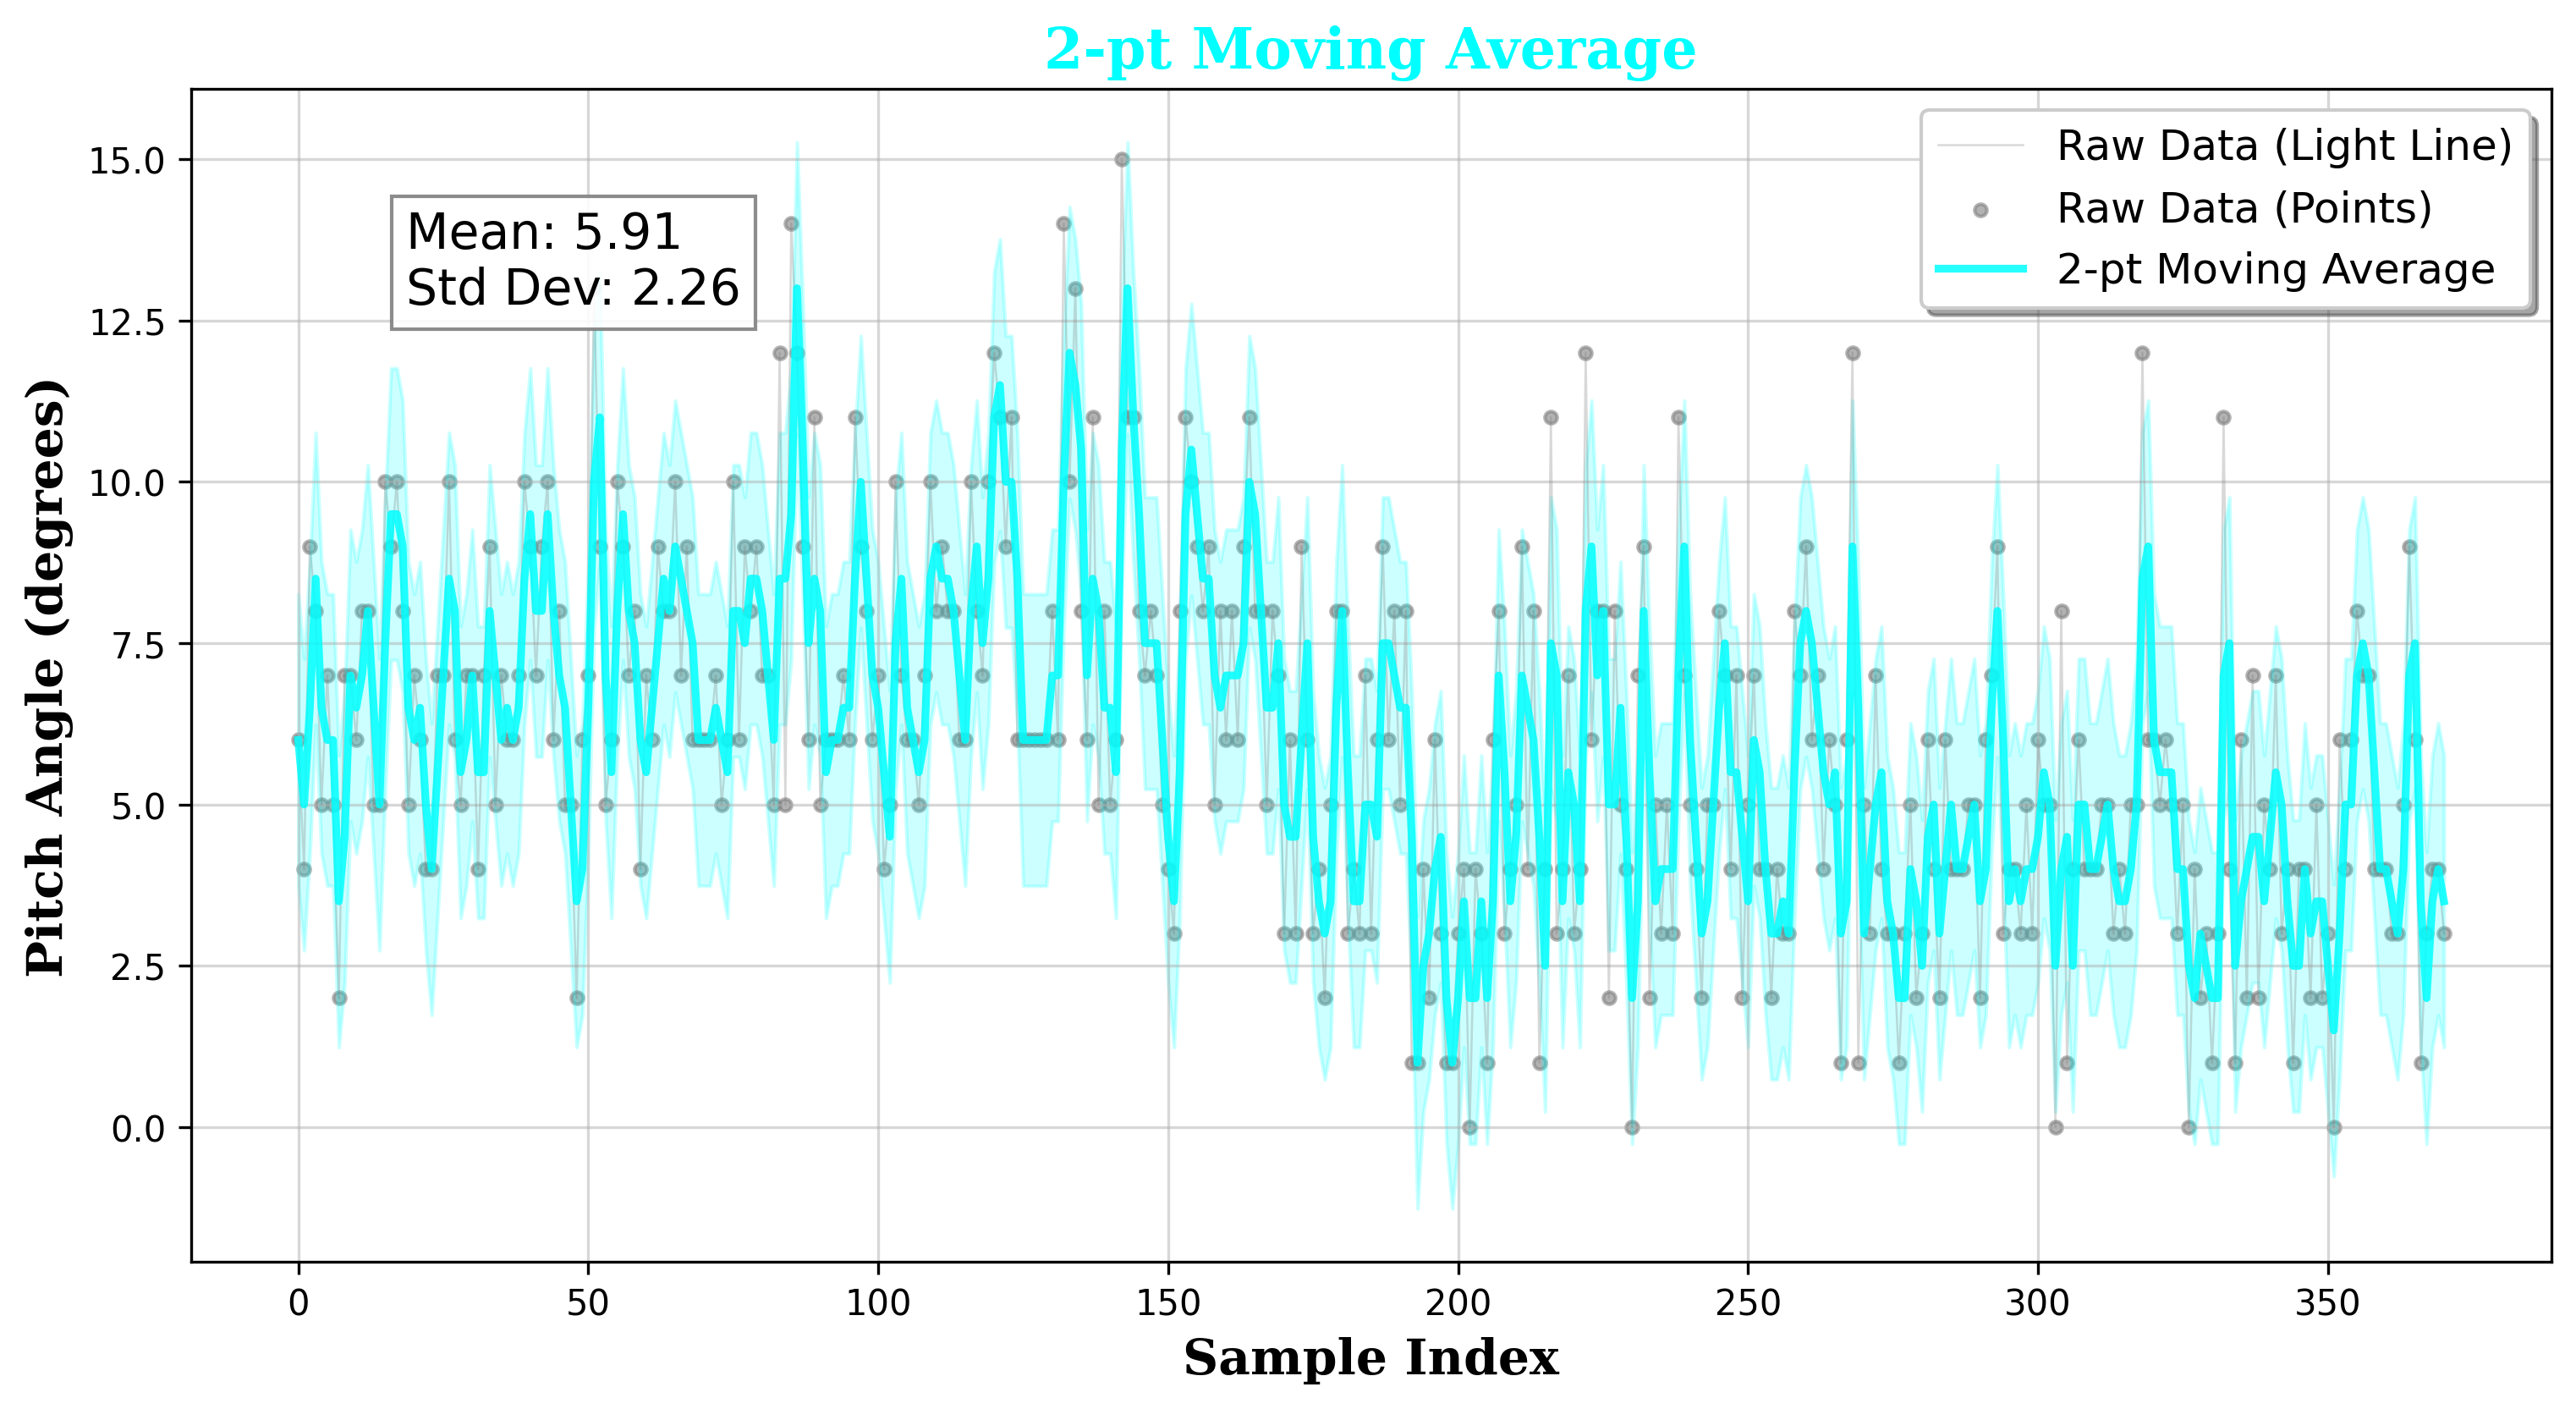
\includegraphics[width=1\textwidth]{pitch_analysis_2pt.png}
    \caption{2-Point Moving Average}
    \label{fig:2pt}
\end{figure}
\begin{figure}[H]
    \centering
    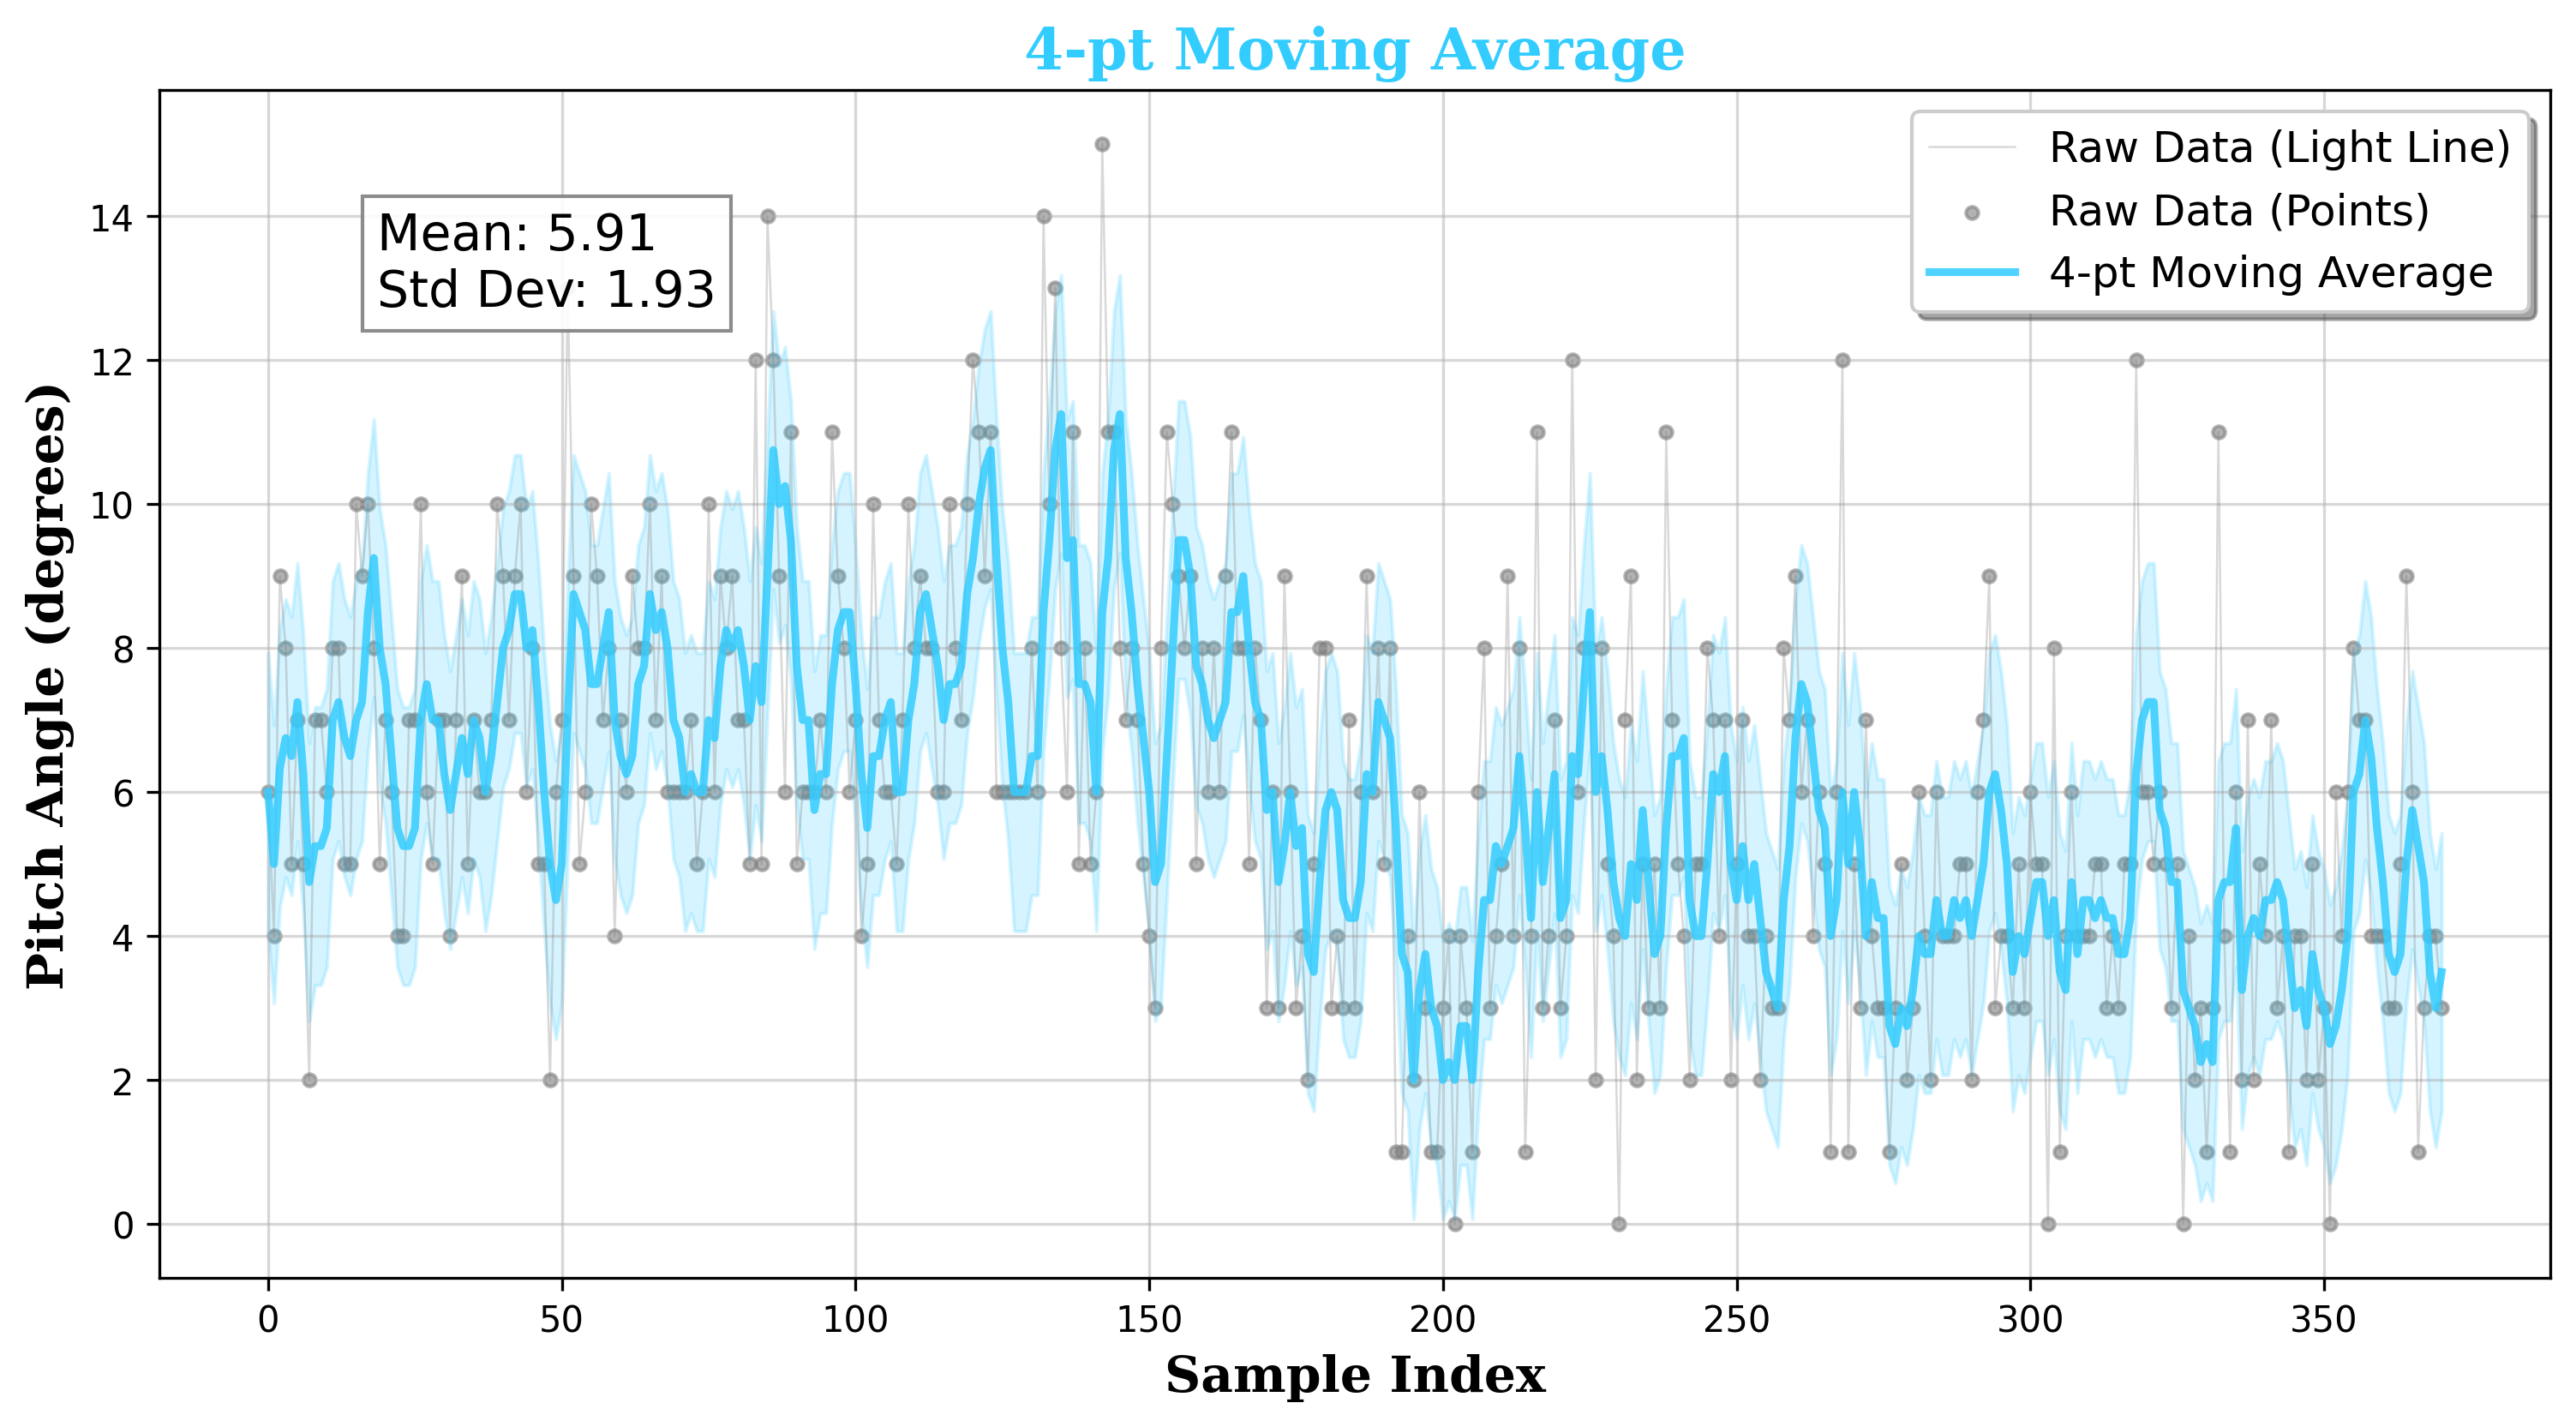
\includegraphics[width=1\linewidth]{pitch_analysis_4pt.png}
    \caption{4-Point Moving Average}
    \label{fig:enter-label}
\end{figure}
\begin{figure}[H]
    \centering
    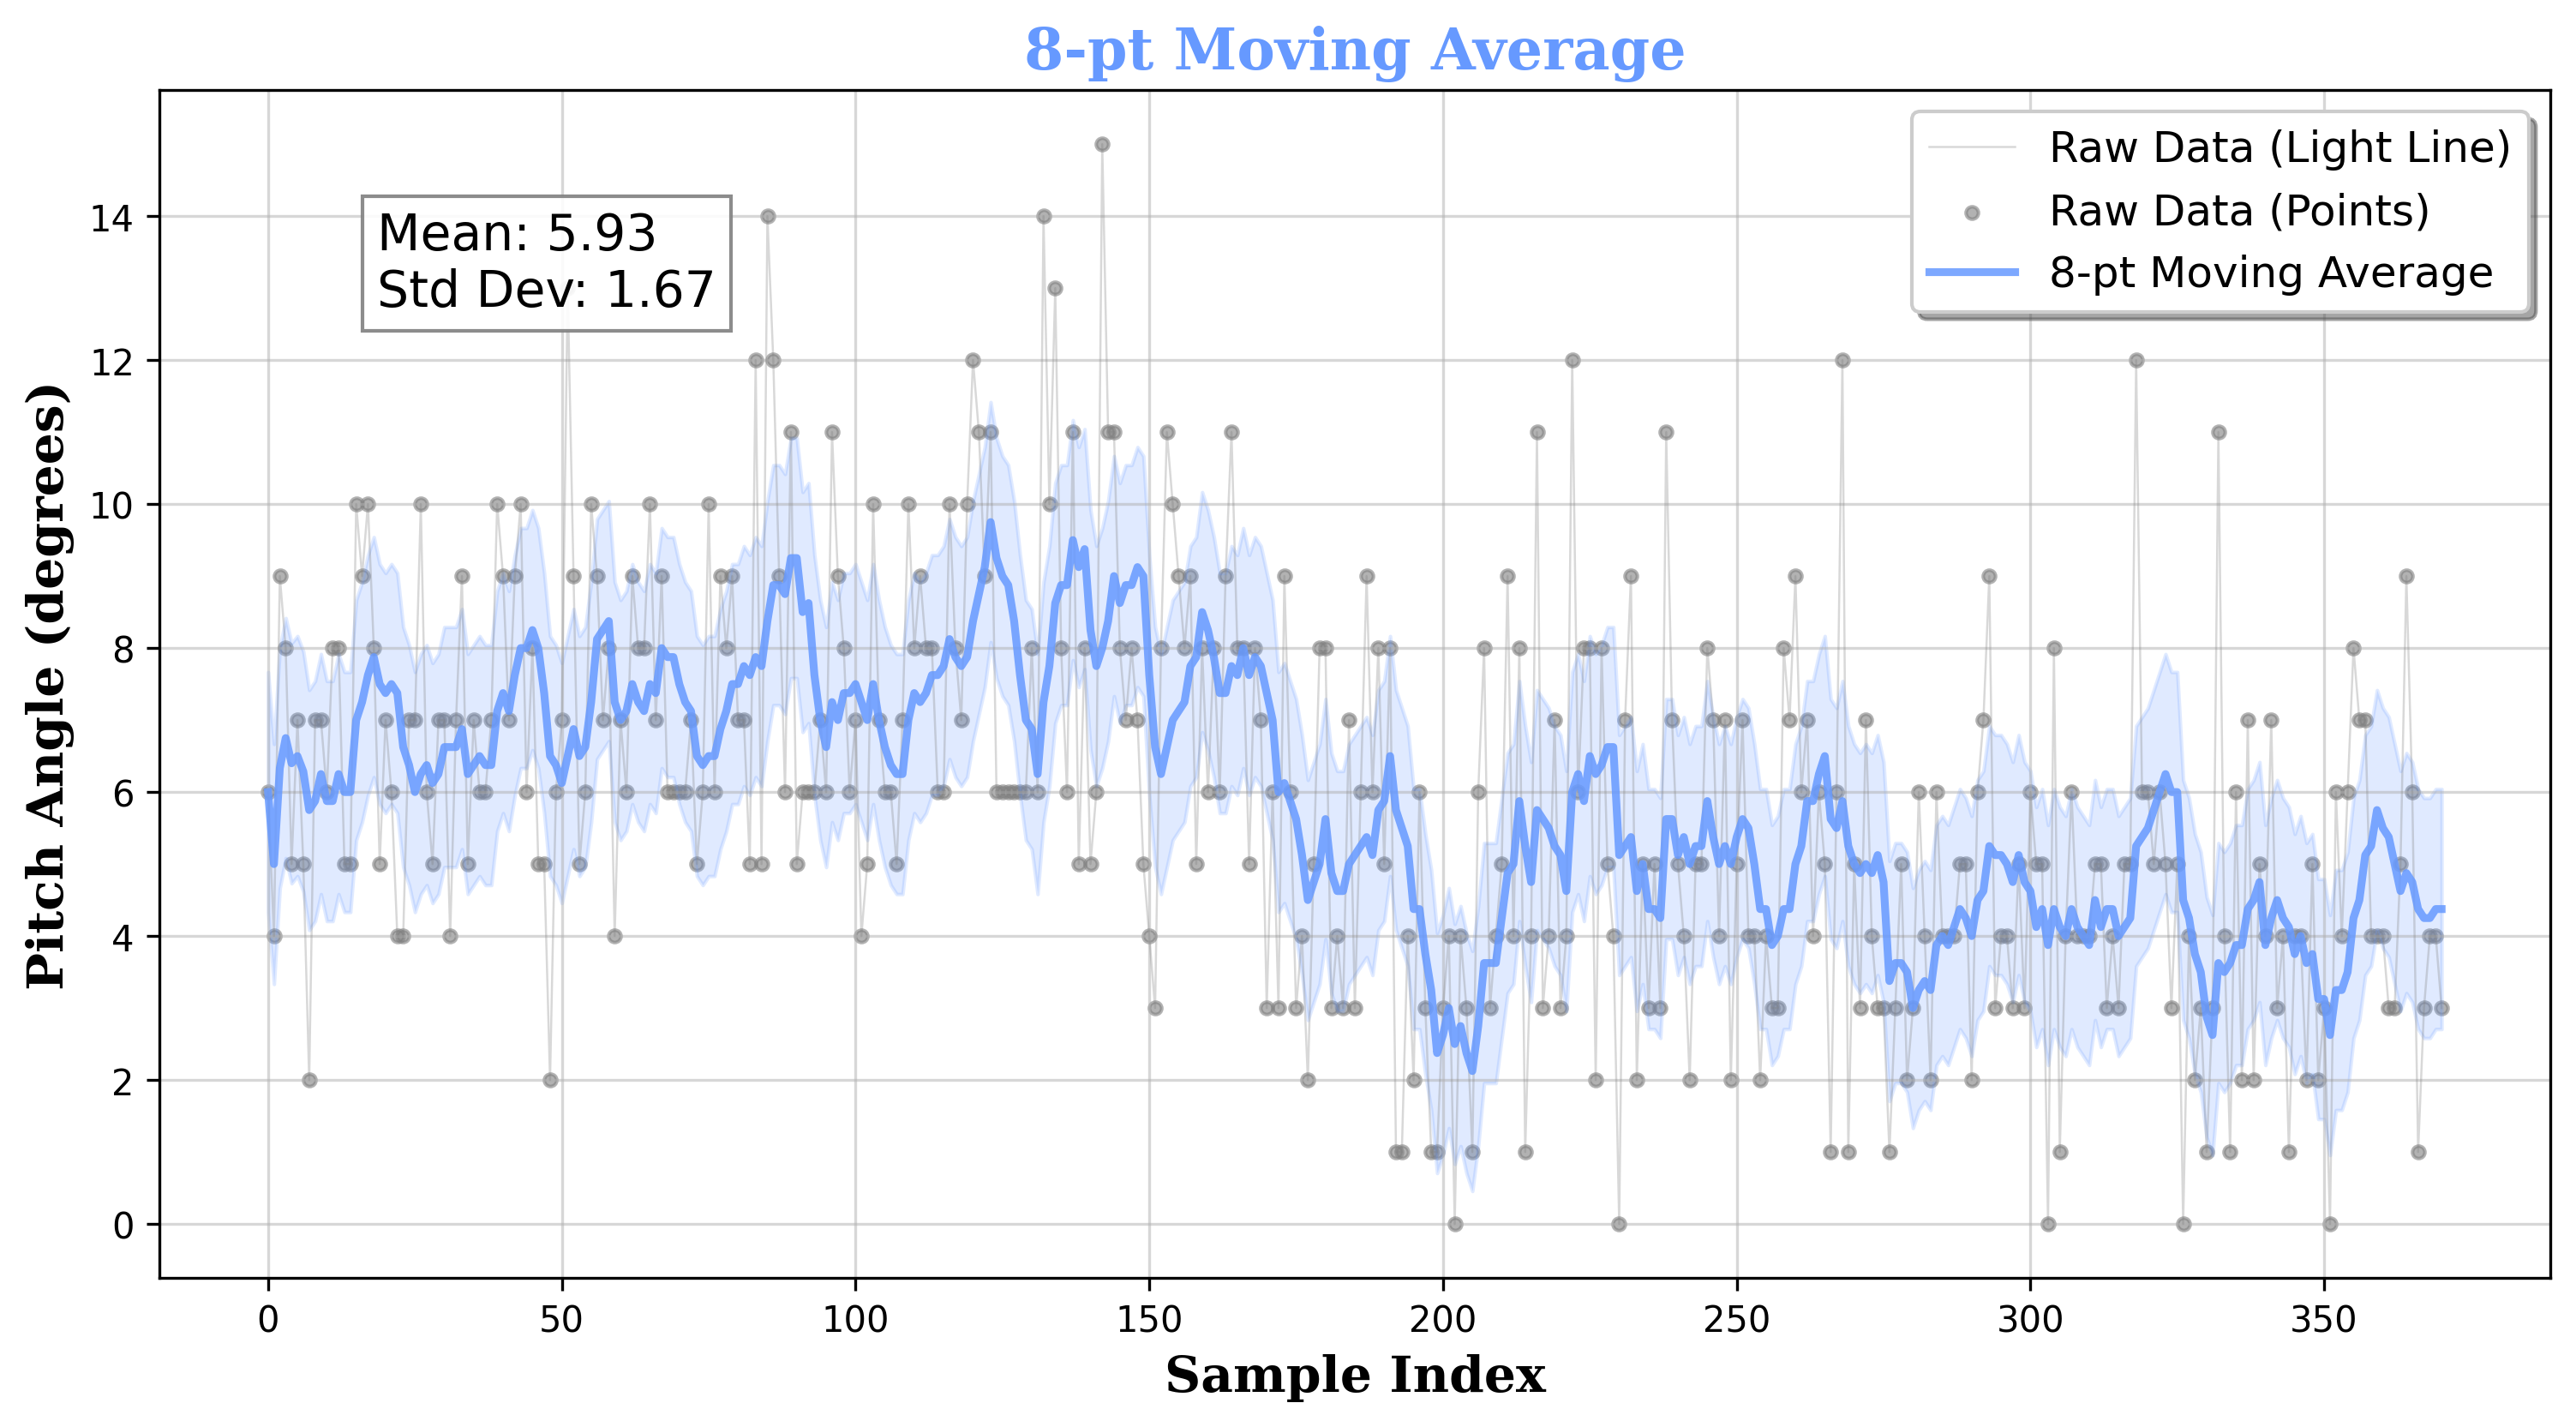
\includegraphics[width=1\linewidth]{pitch_analysis_8pt.png}
    \caption{8-Point Moving Average}
    \label{fig:enter-label}
\end{figure}
\begin{figure}[H]
    \centering
    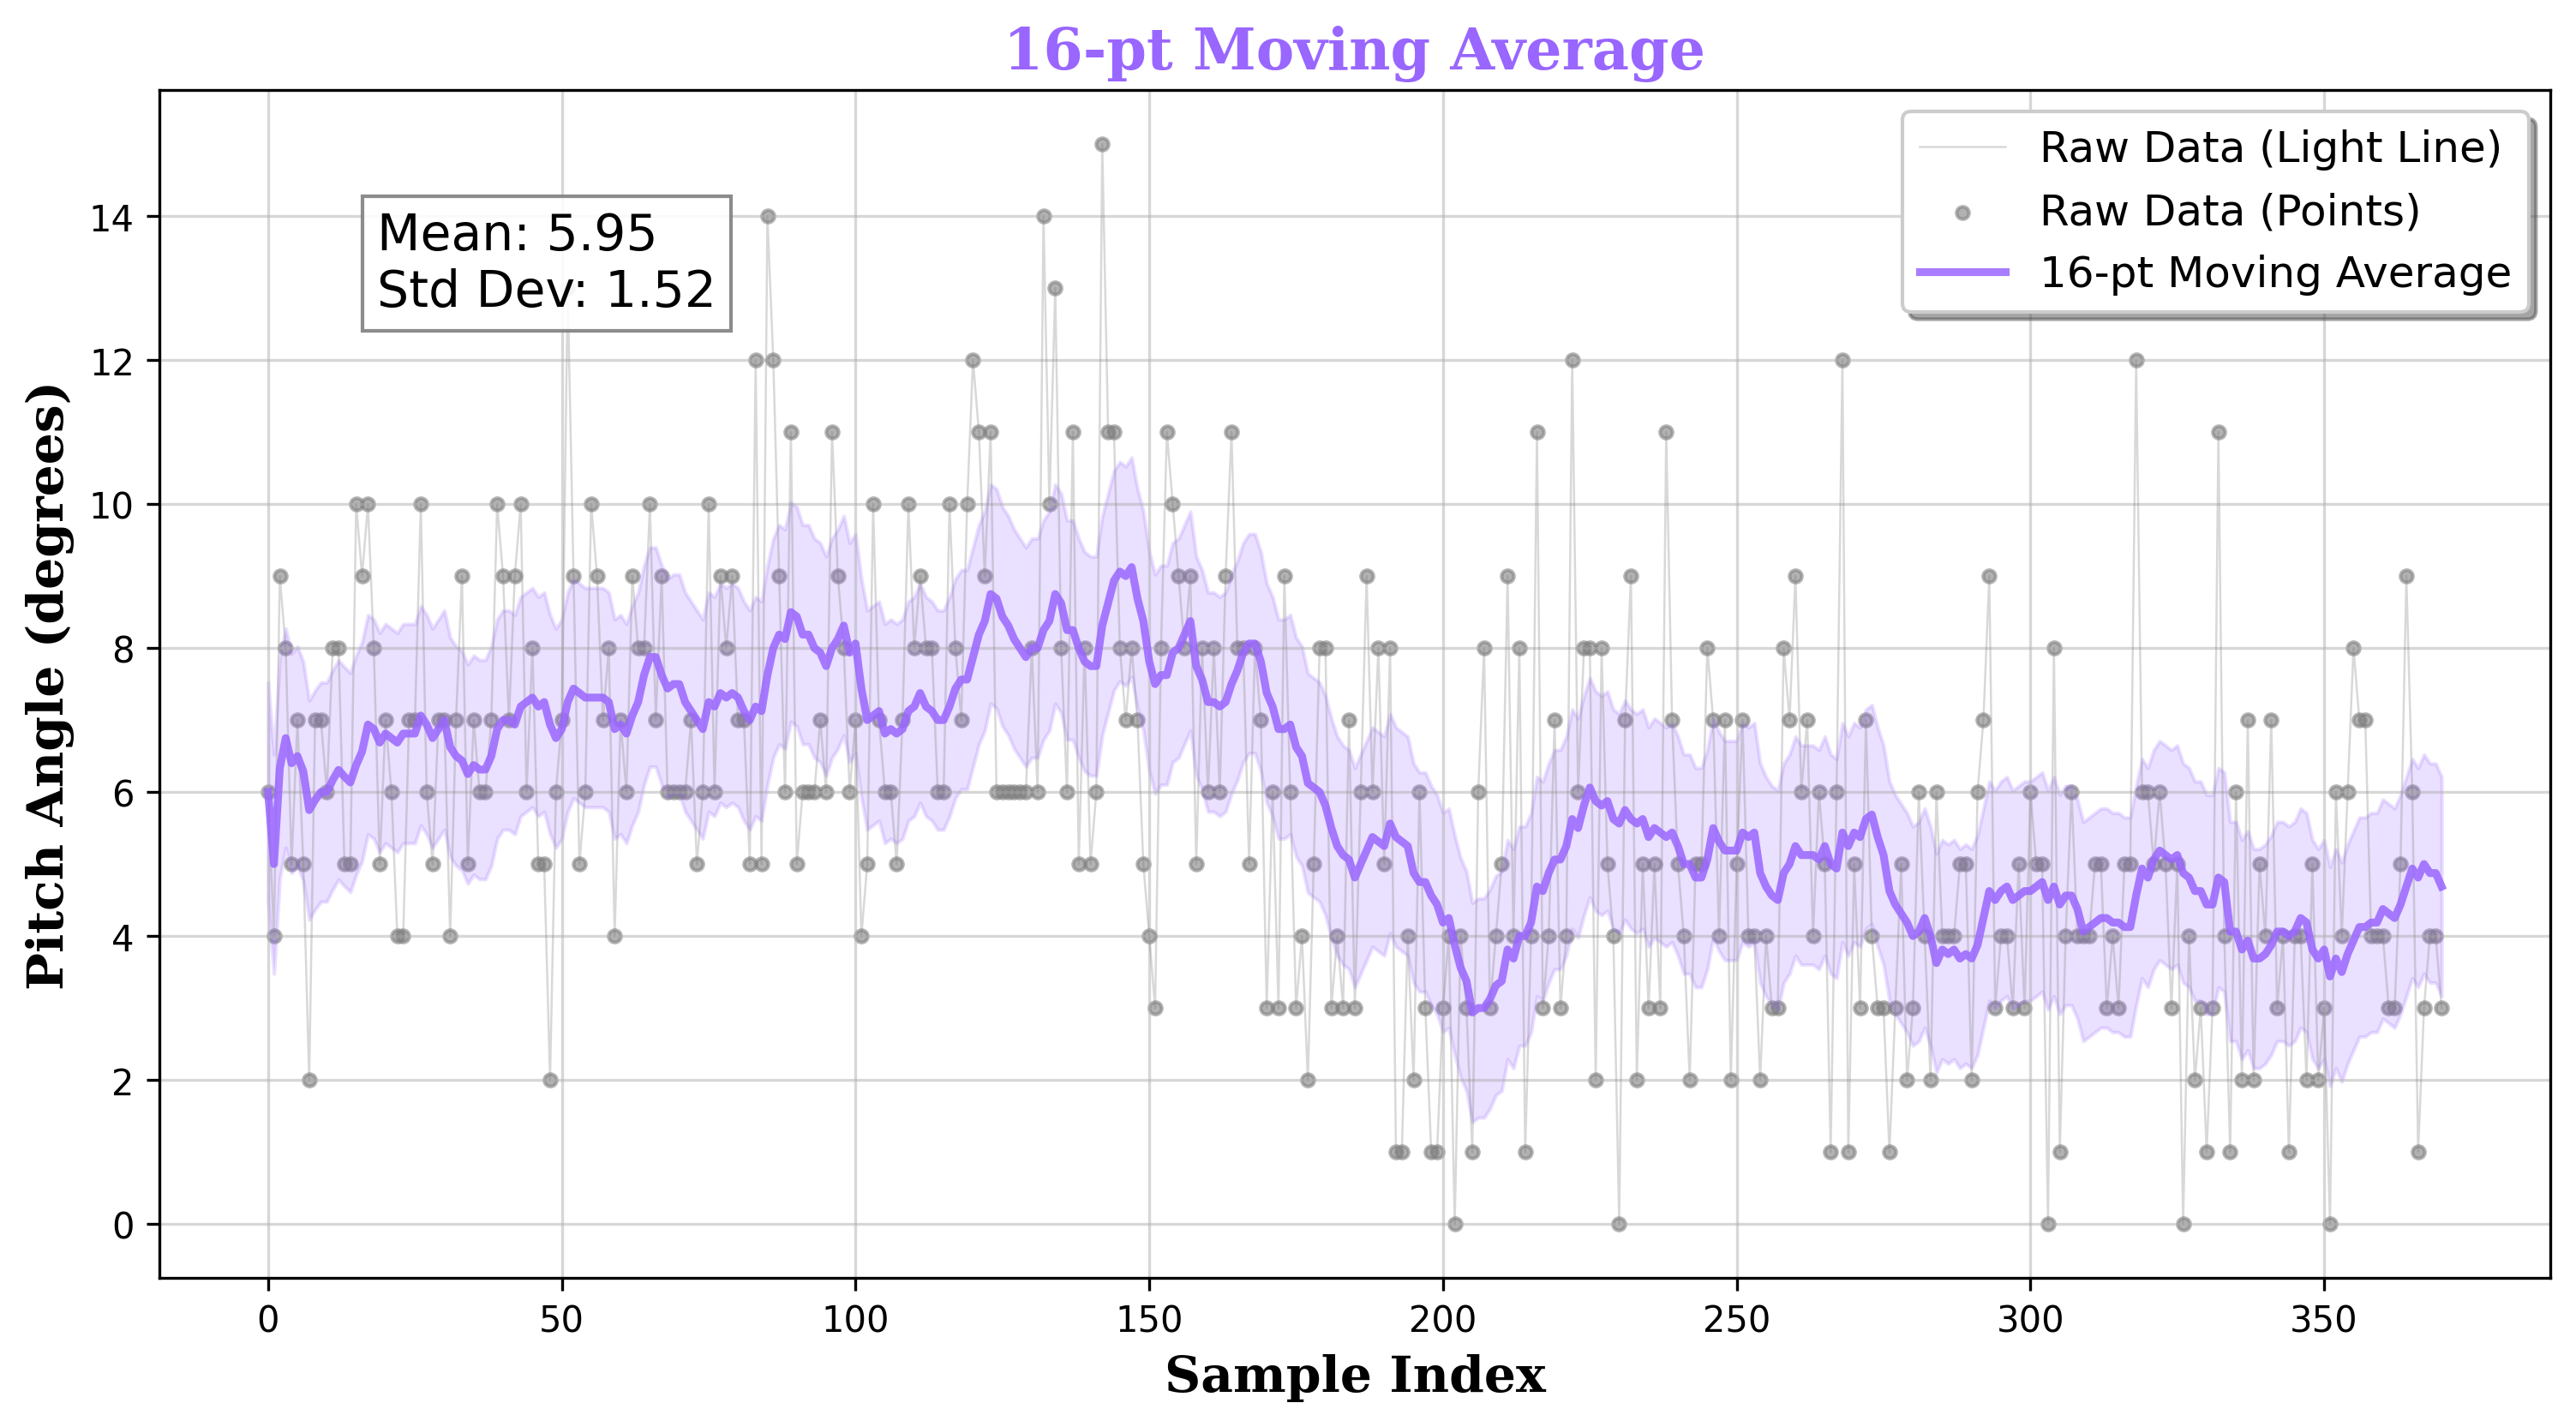
\includegraphics[width=1\linewidth]{pitch_analysis_16pt.png}
    \caption{16-Point Moving Average}
    \label{fig:enter-label}
\end{figure}
\begin{figure}[H]
    \centering
    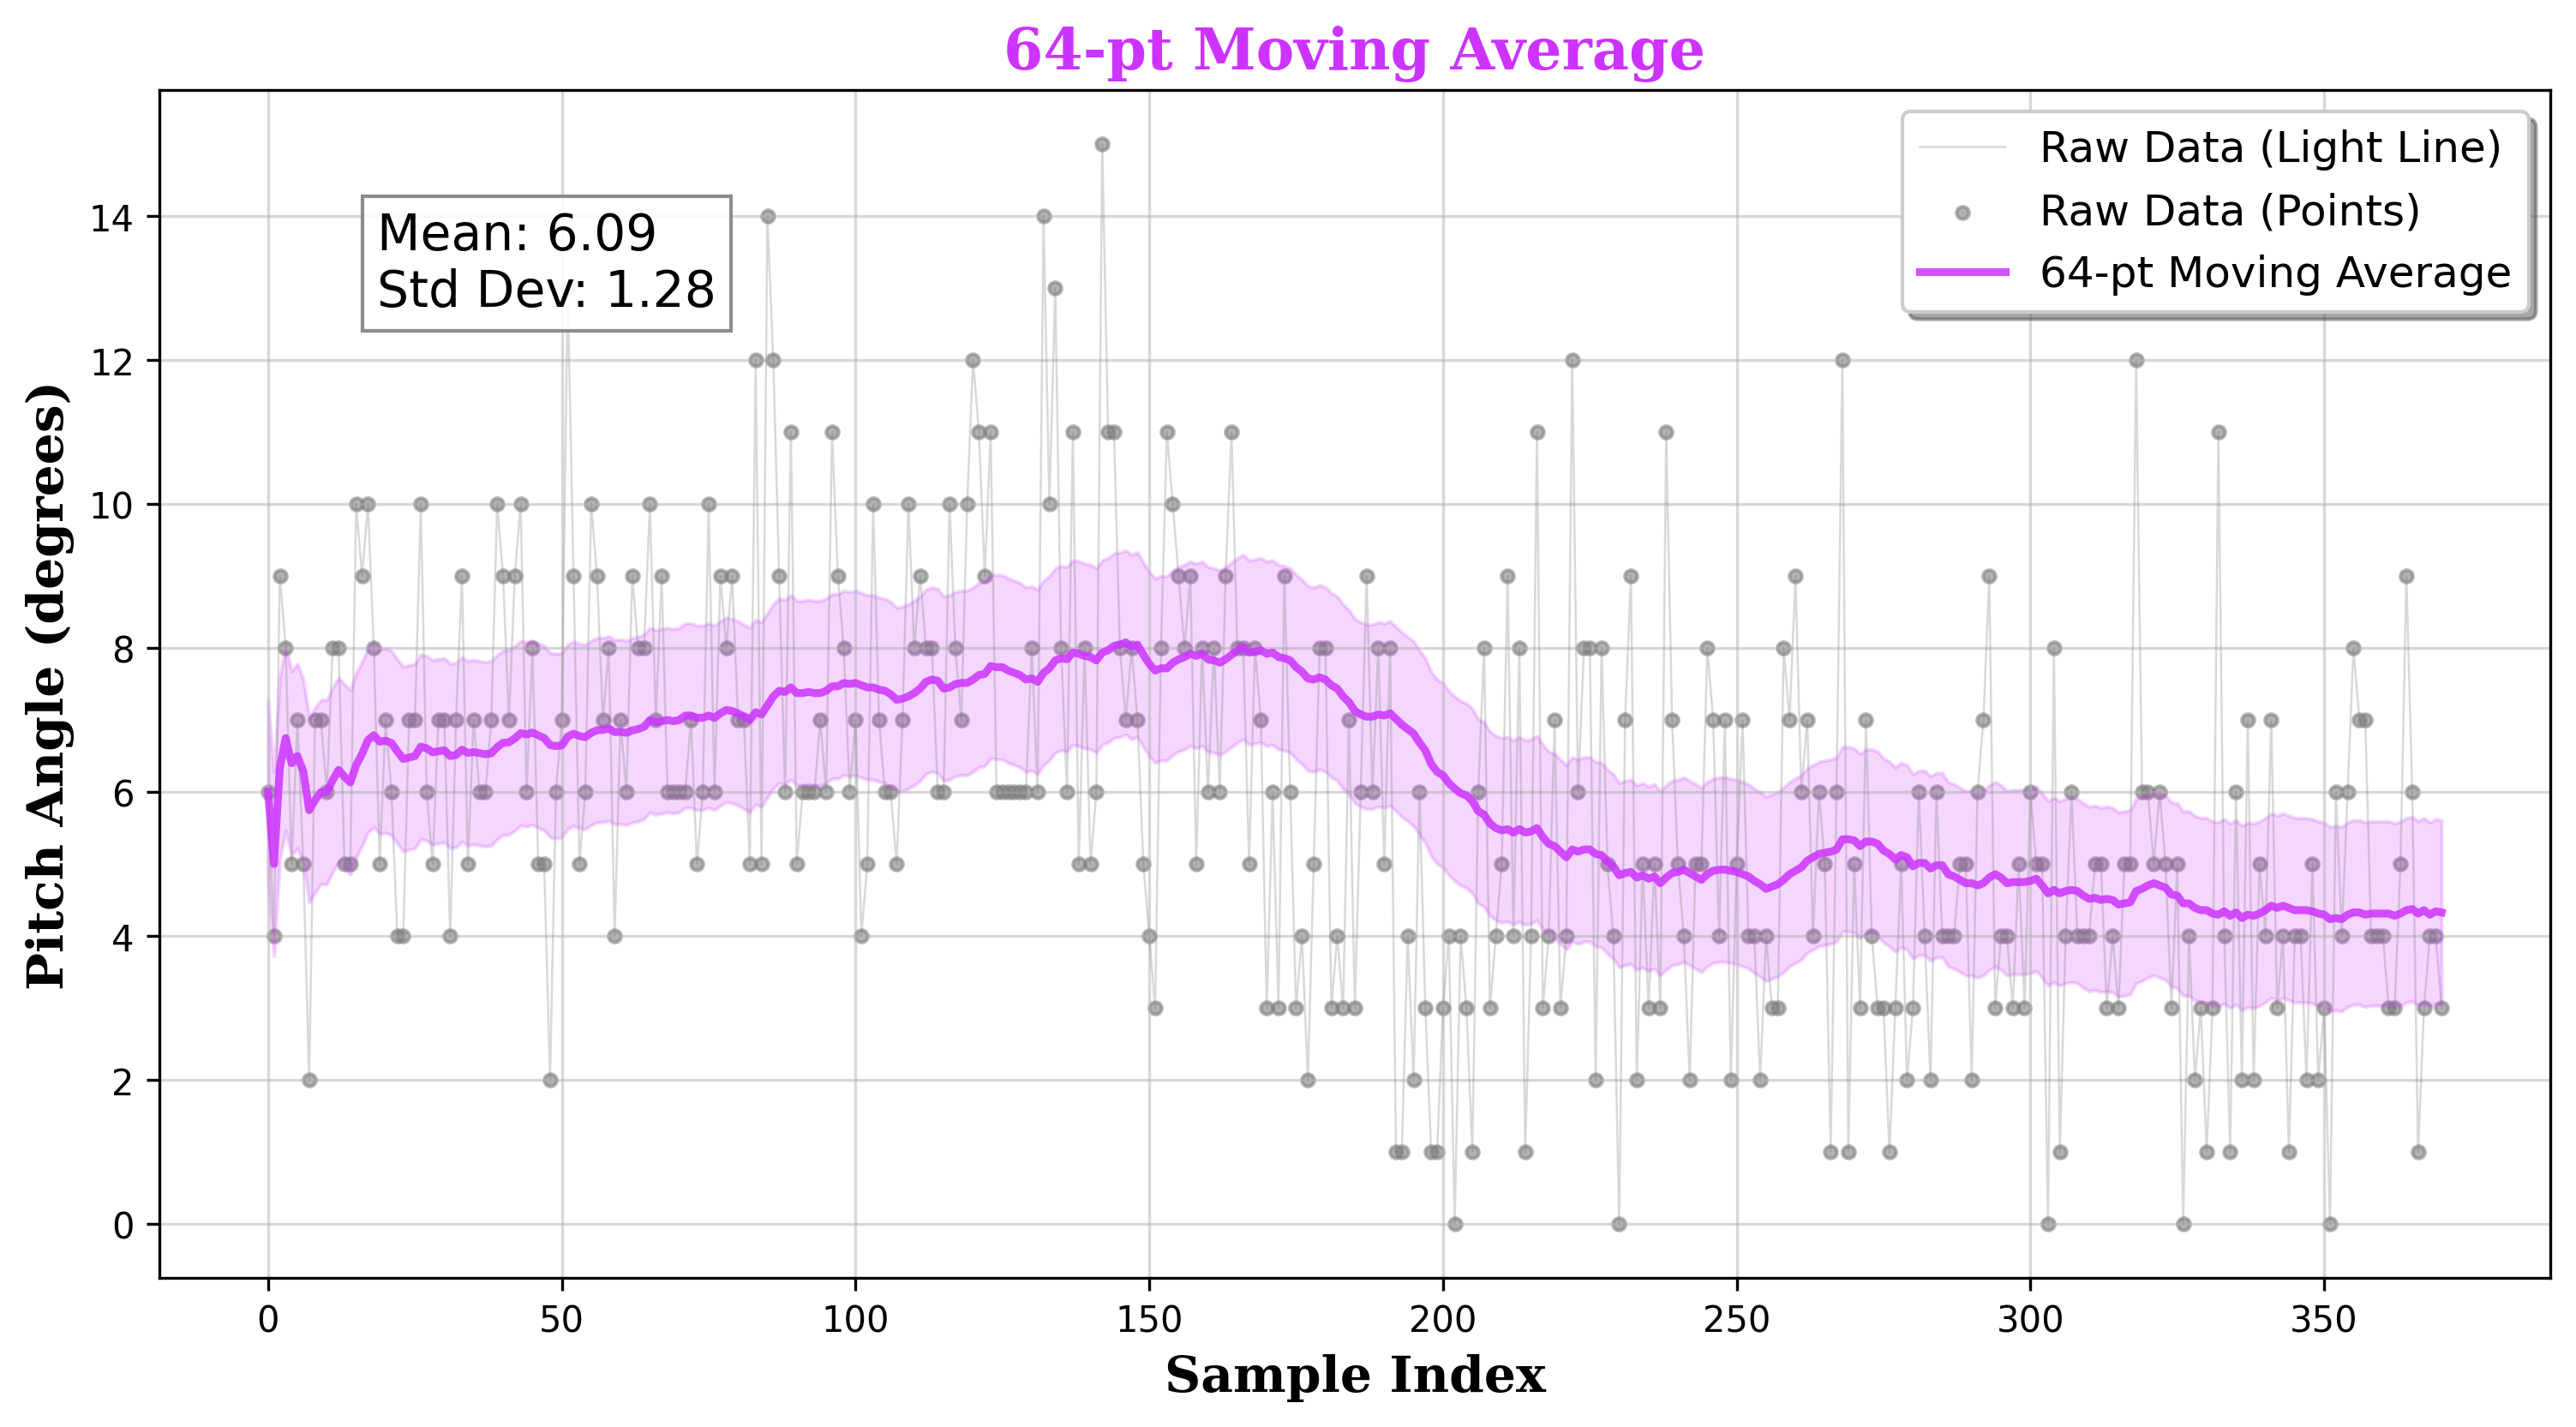
\includegraphics[width=1\linewidth]{pitch_analysis_64pt.png}
    \caption{64-Point Moving Average}
    \label{fig:enter-label}
\end{figure}
\begin{figure}[H]
    \centering
    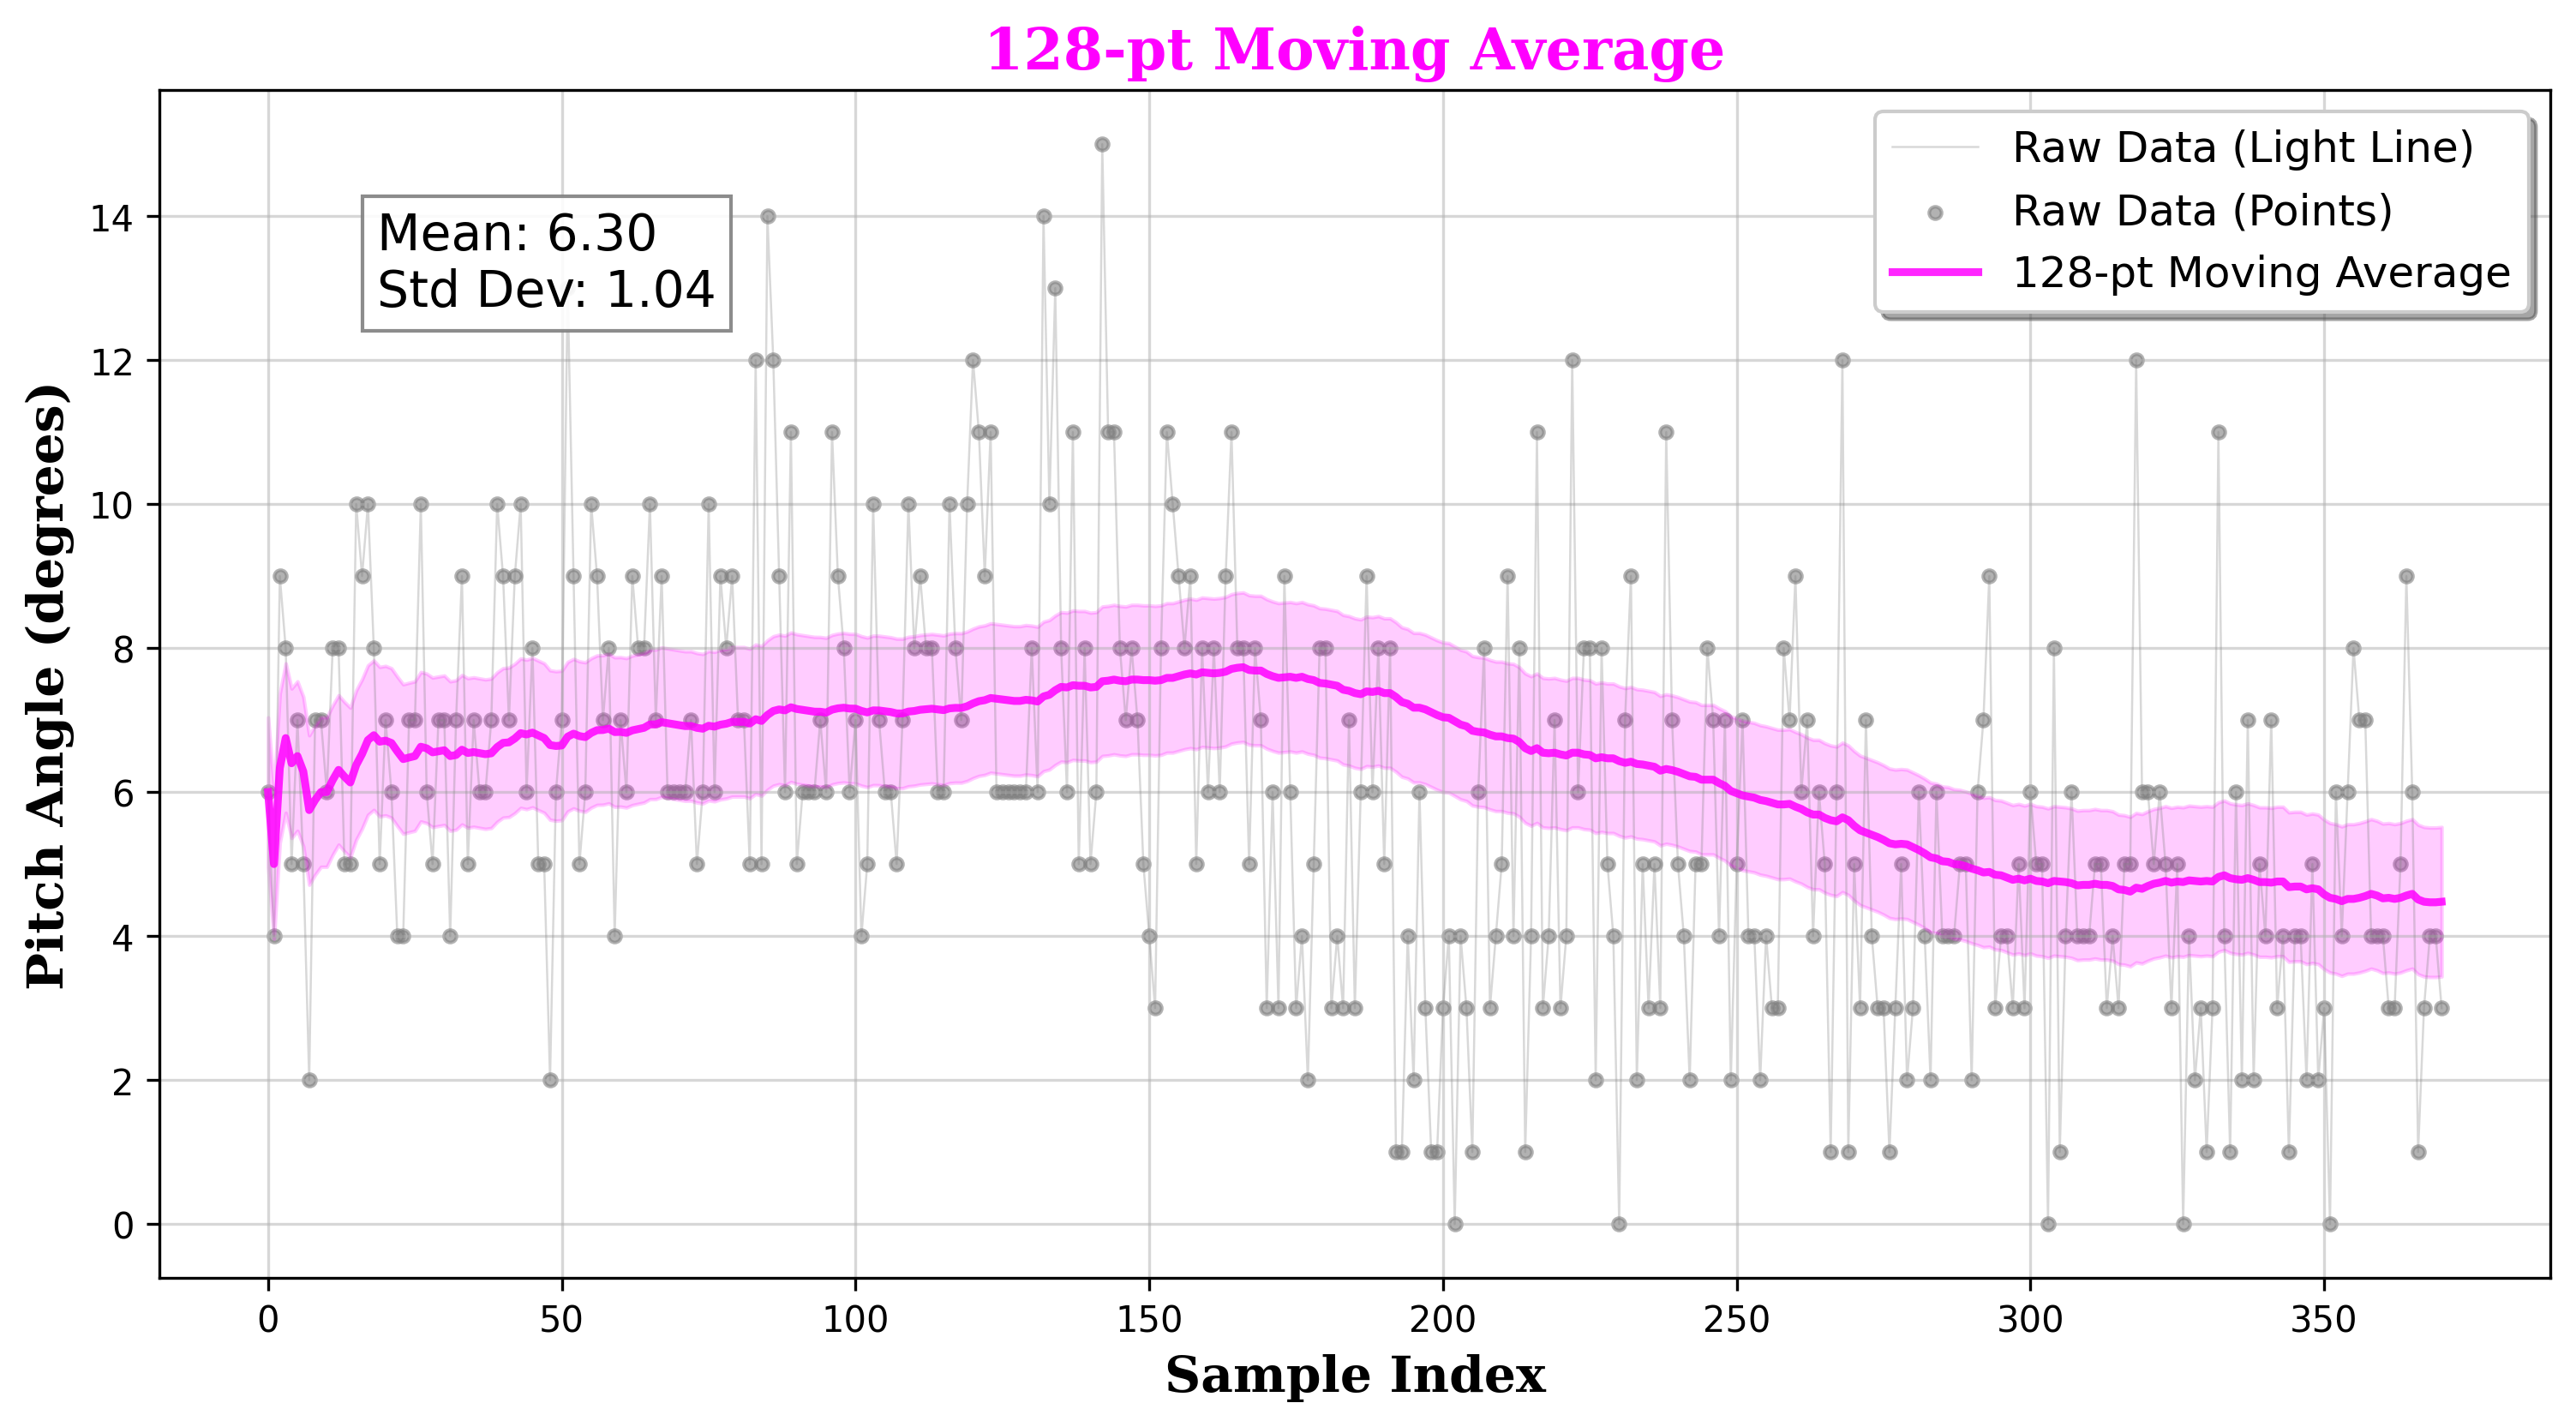
\includegraphics[width=1\textwidth]{pitch_analysis_128pt.png}
    \caption{128-Point Moving Average}
    \label{fig:128pt}
\end{figure}

\section*{Conclusion}
The moving average smooths the raw pitch angle data, reducing noise. Larger window sizes result in greater smoothing but introduce lag. 

The complete code is available at:  
\url{https://github.com/nslaul/ENPM_701_Homework_1}

\end{document}
